%%%%% Remove ? to make this file compilable %%%%%
% TO COMPILE %

%%%%%%%%%%                             %%%%%%%%%%
%%%%%%%%%% AUTO INSERTION D'UNE ENTETE %%%%%%%%%%
%%%%%%%%%%                             %%%%%%%%%%
%%%%%%%%%%     POUR UN FICHIER TEX     %%%%%%%%%%
%%%%%%%%%%                             %%%%%%%%%%

%%%%%%          %%%%%%
%%%%%% PACKAGES %%%%%%
%%%%%%          %%%%%%

\documentclass[8pt]{beamer}
\usepackage[utf8]{inputenc}
\usepackage[english]{babel}
%\usepackage[babel=true,kerning=true]{microtype} % probleme avec : tikz
\usepackage{graphicx}
\usepackage{listings}
\usepackage{color} 
\usepackage{enumerate}
\usepackage{amsfonts}
\usepackage{amssymb}
\usepackage{amsmath}
\usepackage{wasysym}
\usepackage{moreverb}
%\usepackage{chemarrow}
% \usepackage{tikz}
% \usetikzlibrary{positioning}
% \usetikzlibrary{automata}
% \usetikzlibrary{trees}
% \usetikzlibrary{arrows}
\usepackage{beamerthemesplit}
\usetheme{JuanLesPins}


%%%%%%              %%%%%%
%%%%%% MISE EN PAGE %%%%%%
%%%%%%              %%%%%%


%%%%% Environnements %%%%%

% \newenvironment{tikz_mrfou}{
% \begin{tikzpicture}[->,>=stealth,shorten >=1pt,auto,node
%  distance=1.5cm,on grid, semithick, minimum size=5mm,bend
%  angle=10,font=\small, initial text=, label distance=-1mm]
% }{\end{tikzpicture}}

\definecolor{turq}{rgb}{0,0.60,0.60}
\newcommand{\janob}{Jan Obdr\v{z}\`alek}
\newcommand{\coul}[1]{\textcolor{red}{#1}}
\newcommand{\turq}[1]{\textcolor{turq}{#1}}
\newcommand{\magenta}[1]{\textcolor{magenta}{#1}}
\newcommand{\blue}[1]{\textcolor{blue}{#1}}
\newcommand{\Cn}[1]{\textcolor{black}{#1}}

% \tikzstyle{evennode}=[circle,draw=blue!50,fill=blue!20,thick, inner
% sep=0pt,minimum size=6mm]

% \tikzstyle{oddnode}=[rectangle,draw=black!50,fill=black!20,thick, inner
% sep=0pt,minimum size=5mm]


% \tikzstyle{pointnode}=[circle,draw=black,fill=black, thick, inner
% sep=0pt,minimum size=1mm] 

%%%%%%          %%%%%%
%%%%%% DOCUMENT %%%%%%
%%%%%%          %%%%%%


\begin{document}

%%%%%%              %%%%%%
%%%%%% ZONE DE CODE %%%%%%
%%%%%%              %%%%%%

%% Style bloc %%
\setbeamertemplate{blocks}[rounded][shadow=true]
\setbeamercovered{dynamic}

%% Page de garde %%
\author[J. Boyer, D. Cransac, J-S. Dubernet, F. Kuntz - Encadrant :
A. Griffault]{Jérémy Boyer, Dorian Cransac, Jean-Sébastien Dubernet,
Fabien Kuntz\\
~\\
\small Encadrant : Alain Griffault}
\institute{\footnotesize Module PFE\\~\\Master S\&T
Informatique\\~\\Université Bordeaux I\\} 
\title{Projet de fin d'études : \textit{``AltaRica et les robots''}} 
\date{\footnotesize 26 mars 2009}

\setcounter{page}{1}

%% Debut %%
\frame{\titlepage}
\frame{\tableofcontents}

 \section{Introduction}
 %==============================================================================
 \frame{\tableofcontents[current]}
  %==============================================================================
 \begin{frame}
  \frametitle{Le projet}
  
  \begin{block}{Principe}
   \begin{itemize}
    \item Deux robots : Maître et Esclave
	  \uncover<2->{
    \item Robot Maître : capteurs et moteurs}
	  \uncover<3->{
    \item Robot Esclave : seulement moteurs}
	  \uncover<4->{
    \item Maître communique les ordres à l'Esclave par Bluetooth}
	  \uncover<5->{
    \item Esclave : pas de décision}
   \end{itemize}
  \end{block}

  \uncover<6->{
  \begin{block}{But}
   \begin{itemize}
    \item Accomplir une mission non triviale mettant en jeu les deux robots
	  \uncover<7->{
    \item Vérifier cette mission en modélisant en Altarica}
    \uncover<8->{
    \item Etudier la possibilité d'une generation de code automatique}
   \end{itemize}
  \end{block}
  }

 \end{frame}


 \section{Mission}
 %==============================================================================
 \frame{\tableofcontents[current]}

%  \include{paritygame}
%  \include{cliquewidth}

 \section{Modèle AltaRica}
 %==============================================================================
 \frame{\tableofcontents[current]}
   
    \section{AltaRica}

  \subsection{Architecture}
  \begin{figure}[!ht]
   \begin{center}
    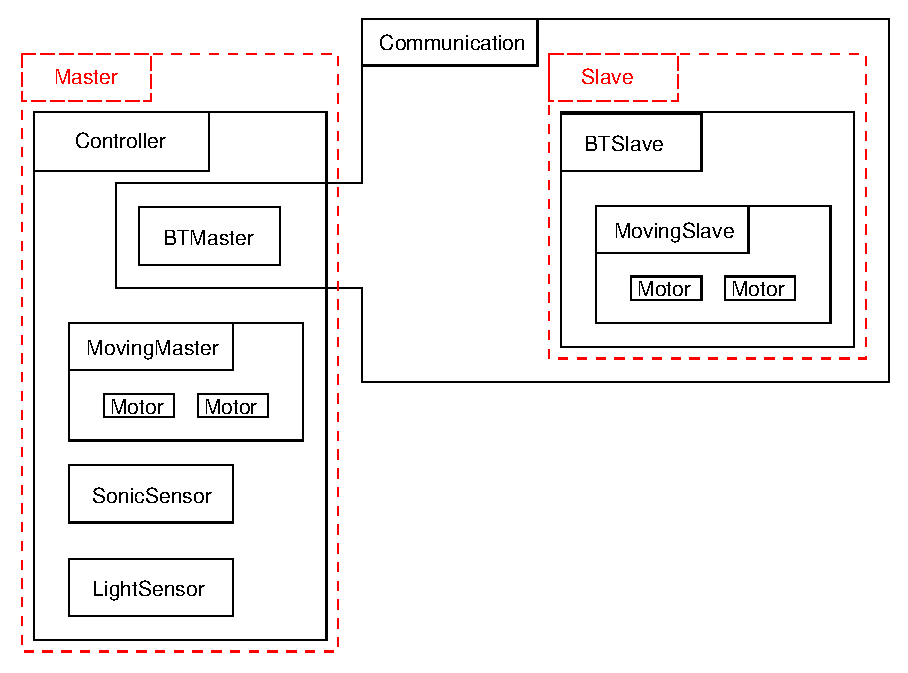
\includegraphics{ARmodel.eps}
    \caption{Architecture AltaRica}
   \end{center}
  \end{figure}

  \subsection{Les capteurs et moteurs}
    
   \subsubsection{Le n\oe{}ud LightSensor}

    \paragraph{\underline{Description\\}}
    Ce noeud correspond au capteur de lumière, et possède une variable
    d'état nommée $color$ qui   peux prendre trois valeurs différentes,
    correspondants au trois couleurs de case que nous allons utiliser:
    Noir, gris et blanc. Cette variable d'état n'est présente que pour
    pouvoir modéliser des événements, qui seront déclenché par les
    différentes valeurs de la variable de flux $value$. L'action du
    senseur de lumière est donc véritablement représentée par cette
    variable de flux, puisque les valeurs lues par le senseur sont
    "incontrôlables".

    \paragraph{\underline{Le source Altarica\\}}
    \verbatiminput{../src/altarica/alt/LightSensor.alt}
   
    \paragraph{\underline{La spécification\\}}
    \verbatiminput{../src/altarica/acheck/LightSensor.acheck}

    \paragraph{\underline{La sémantique\\}}
    \begin{figure}[!ht]
     \begin{center}
      \includegraphics{../src/altarica/LightSensor.eps}
      \caption{LightSensor}
     \end{center}
    \end{figure}

    \paragraph{\underline{Les résultats\\}}
    \verbatiminput{../src/altarica/LightSensor.prop}
    \verbatiminput{../src/altarica/LightSensor.res}
   
   \subsubsection{Le n\oe{}ud UltraSonicSensor}
   
    \paragraph{\underline{Description\\}}
    De la même manière que le noeud LightSensor, UltraSonicSensor
    comporte une variable d'état "behind" qui servira à pouvoir
    déclencher les deux évènements $readValue$. Le principe du capteur
    est que soit il y a un objet capté, soit il n'y en a pas, sans
    distinction véritable de distance. Et comme pour LightSensor, c'est
    la variable de flux $d$ qui déclenche ces évènements.

    \paragraph{\underline{Le source Altarica\\}}
    \verbatiminput{../src/altarica/alt/UltraSonicSensor.alt}
    
    \paragraph{\underline{La spécification\\}}
    \verbatiminput{../src/altarica/acheck/UltraSonicSensor.acheck}
    
    \paragraph{\underline{La sémantique\\}}
    \begin{figure}[!ht]
     \begin{center}
      \includegraphics{../src/altarica/UltraSonicSensor.eps}
      \caption{UltraSonicSensor}
     \end{center}
    \end{figure}

    \paragraph{\underline{Les résultats\\}}
    \verbatiminput{../src/altarica/UltraSonicSensor.prop}
    \verbatiminput{../src/altarica/UltraSonicSensor.res}
   
   \subsubsection{Le n\oe{}ud Motor}
  
    \paragraph{\underline{Description\\}}
    Les moteurs sont modélisés de façon à avoir seulement trois vitesses
    possible: Avancer, stopper, reculer.

    \paragraph{\underline{Le source Altarica\\}}
    \verbatiminput{../src/altarica/alt/Motor.alt}
    
    \paragraph{\underline{La spécification\\}}
    \verbatiminput{../src/altarica/acheck/Motor.acheck}
    
    \paragraph{\underline{La sémantique\\}}
    \begin{figure}[!ht]
     \begin{center}
      \includegraphics{../src/altarica/Motor.eps}
      \caption{Motor}
     \end{center}
    \end{figure}

    \paragraph{\underline{Les résultats\\}}
    \verbatiminput{../src/altarica/Motor.prop}
    \verbatiminput{../src/altarica/Motor.res}
   
  \subsection{Les déplacements, n\oe{uds Moving}}

    \paragraph{\underline{Description\\}}
    Les n\oe{}uds Moving sont là pour faire la synchronisation entre les deux moteurs
    munis de roues d'un robot. Il y a cinq ordres possible: Avancer,
    s'arrêter, reculer, à droite et à gauche. Il faut savoir que les
    rotations à droite et à gauche du robot sont tout le temps de 90
    degrés.

    \paragraph{\underline{Les sources Altarica\\}}
    \verbatiminput{../src/altarica/alt/MovingMaster.alt}
    \verbatiminput{../src/altarica/alt/MovingSlave.alt}
    
    \paragraph{\underline{Les spécifications\\}}
    \verbatiminput{../src/altarica/acheck/MovingMaster.acheck}
    \verbatiminput{../src/altarica/acheck/MovingSlave.acheck}
    
    \paragraph{\underline{La sémantique\\}}
    \begin{figure}[!ht]
     \begin{center}
      \includegraphics[width=16cm]{../src/altarica/MovingMaster.eps}
      \caption{MovingMaster}
     \end{center}
    \end{figure}

    \begin{figure}[!ht]
     \begin{center}
      \includegraphics[width=16cm]{../src/altarica/MovingSlave.eps}
      \caption{MovingSlave}
     \end{center}
    \end{figure}

    \paragraph{\underline{Les résultats\\}}
    \verbatiminput{../src/altarica/MovingMaster.prop}
    \verbatiminput{../src/altarica/MovingMaster.res}
    ~\newline
    \verbatiminput{../src/altarica/MovingSlave.prop}
    \verbatiminput{../src/altarica/MovingSlave.res}
    
  \subsection{La communication}
    
   \subsubsection{Les n\oe{}uds BTMaster, BTSlave et MasterSlave}
    
    \paragraph{\underline{Description\\}}
    La communication bluetooth entre les deux robots est de type
    maitre/esclave, le maitre envoie simplement des ordres à executer à
    l'esclave. Le noeud BTMaster qui sera pour le robot maitre comporte
    donc simplement les cinq même ordres que le noeud moving. BTSlave
    sera lui pour le robot esclave, et inclus un sous noeud de type
    Moving, afin de pouvoir synchroniser les cinq ordres possibles à un
    agissement concret de ce noeud Moving. Enfin, le noeud MasterSlave se
    chargera de faire la synchronisation entre les ordres des noeuds
    BTMaster et BTSlave.

    \paragraph{\underline{Les sources Altarica\\}}
    \verbatiminput{../src/altarica/alt/BTMaster.alt}
    \verbatiminput{../src/altarica/alt/BTSlave.alt}
    \verbatiminput{../src/altarica/alt/BTMasterSlave.alt}
    
    \paragraph{\underline{Les spécifications\\}}
    \verbatiminput{../src/altarica/acheck/BTMaster.acheck}
    \verbatiminput{../src/altarica/acheck/BTSlave.acheck}
    \verbatiminput{../src/altarica/acheck/BTMasterSlave.acheck}

    \paragraph{\underline{La sémantique}}
    \begin{figure}[!ht]
     \begin{center}
      \includegraphics[width=16cm]{../src/altarica/BTMaster.eps}
      \caption{BTMaster}
     \end{center}
    \end{figure}
    \begin{figure}[!ht]
     \begin{center}
      \includegraphics[width=16cm]{../src/altarica/BTSlave.eps}
      \caption{BTSlave}
     \end{center}
    \end{figure}
    \begin{figure}[!ht]
     \begin{center}
      \includegraphics[width=16cm]{../src/altarica/BTMasterSlave.eps}
      \caption{BTMasterSlave}
     \end{center}
    \end{figure}
   
  \subsection{Le n\oe{}ud Controller}
   
    \paragraph{\underline{Le source Altarica\\}}
    \verbatiminput{../src/altarica/alt/Controller.alt}
    
    \paragraph{\underline{La spécification\\}}
    \verbatiminput{../src/altarica/acheck/Controller.acheck}
    
    \paragraph{\underline{La sémantique\\}}
    \begin{figure}[!ht]
     \begin{center}
      
\includegraphics[width=16cm]{../src/altarica/Controller.eps}
      \caption{Controller}
     \end{center}
    \end{figure}

    \paragraph{\underline{Les résultats\\}}
    \verbatiminput{../src/altarica/Controller.prop}
    \verbatiminput{../src/altarica/Controller.res}

%  \include{principe}
%  \include{examplealgo}
  
 \section{Implémentation}
 %==============================================================================
 \frame{\tableofcontents[current]}

%  \include{principe}
%  \include{examplealgo}

 \section{Bilan}
 %==============================================================================
 \frame{\tableofcontents[current]}

 \begin{frame}

  \begin{block}{Bilan}
   \begin{center}
    Nous venons de voir qu'après les jeux de parité à largeur de DAG
    bornée et ceux à largeur d'arbre bornée, un nouveau type de jeu de
    parité est désormais soluble en temps polynomial : ceux à largeur de
    clique bornée.
   \end{center}
  \end{block}

  \pause
  \begin{block}{Question}
   \begin{center}
    En utilisant cette méthode, en élargissant petit à petit le type de
    jeu de parité considéré, ou même en cherchant d'autres opérations de
    construction de graphes, ne pourrions-nous pas finalement réussir à 
    trouver un algorithme polynomial pour résoudre tous les jeux de 
    parité, et ainsi répondre à cette grande question de complexité ?
   \end{center}
  \end{block}

 \end{frame}

 \section*{Références}
 \begin{frame}[allowframebreaks]
  \frametitle{Quelques références}
%   \nocite{*}
%   \bibliographystyle{alpha}
%   \bibliography{biblio}
 \end{frame}

%%%%%%               %%%%%%
%%%%%% /ZONE DE CODE %%%%%%
%%%%%%               %%%%%%

\end{document}



%%%%%%           %%%%%%
%%%%%% /DOCUMENT %%%%%%
%%%%%%           %%%%%%




%%%%% Texte italique %%%%%
%  \textit{} 

%%%%% Liste %%%%
%%% Itemize %%%
%  \begin{itemize}
%   \item item1\\
%   \item item2
%  \end{itemize}

%%% Enumerate %%%
%  \begin{enumerate}
%   \item item1
%   \item item2
%  \end{enumerate}

%%%%% Tabulations %%%%%
%   \begin{tabbing}
%    XX\=XX\=\kill
%    \>(OrdresEnonce.v, ligne 244)\\
%    \>\>test2
%   \end{tabbing}
 
%%%%% Note de pied de page %%%%%
%  \footnote{test}

%%%%% Référence %%%%%
%   \label{ref}
%% Plus loin :
%   \ref{ref}
%   \pageref{ref}

%%%%% Code %%%%%
% \begin{lstlisting}
%      List<Integer> lexBFS2 = new ArrayList<Integer>();
%      lexBFS2.add(3);
%      lexBFS2.add(2);
%      lexBFS2.add(4);
%      lexBFS2.add(1);
%      lexBFS2.add(0);    
%      assertNotNull(lexBFS2);	
%      assertEquals(lexBFS2,Graphs.lexBFS(nogYComp));
%   \end{lstlisting}

%%%%% Inclure une figure %%%%%
%  \begin{figure}[!ht]
%   \begin{center}
%	\includegraphics[width=7cm]{figs/cours1/fig2.eps}
%	\caption{\emph{MT2} : Calcul non déterministe}
%   \end{center}
%  \end{figure}

%%%%% Dessiner une figure %%%%% 
%   \begin{center}
%    \begin{tikz_mrfou}

%     %% Nodes %%
%     \node[state, initial] (1) {$1$};
%     \node[state, right of=1] (2) {$2$};
%     \node[state, right of=2] (3) {$3$};

%     %% Edges %%
%     \path[->] 
%     (1) 
%     edge [loop above] node {b} ()
%     edge node {a} (2)

%     (2)
%     edge [loop above] node {b} ()
%     edge [bend left] node {a} (3)

%     (3)
%     edge [bend left] node {b} (2);

%    \end{tikz_mrfou}
%   \end{center}
